% !TeX spellcheck = hu_HU
% !TeX encoding = UTF-8

% TODO: struktúra meghatározása
\chapter{Virtualizációs környezet létrehozása}
\label{chap:testenv}

\section{Kialakítani kívánt környezet meghatározása}
Dolgozatomban egy kisebb léptékű, de a fontosabb elvek ismertetését kellő mértékben lehetővé tevő tesztkörnyezetet fogok kialakítani és részletesen bemutatni. A tesztkörnyezetben egy fizikai gépen (virtual host) fogok virtuális gépeket kialakítani a \acrshort{kvm} \gls{hypervisor} és a \gls{libvirt} virtualizációs \acrshort{api} segítségével. Ezen környezet célja, hogy betekintést engedjen a nagyvállalati környezetekben alkalmazott virtualizációs rendszerek kialakításának fontosabb lépéseibe.

A \acrshort{kvm}-re és a \gls{libvirt}-re azért esett a választásom, mert ezek modern technológiáknak tekinthetőek, az elmúlt 20 évben jöttek létre, és a mai napig aktívan fejlesztik őket. A \acrshort{kvm} a Linux kernel része, így a támogatottsága egyedülálló, és lényegében minden Linux disztribúción használható. Emellett több nagy szoftvergyártó és felhőszolgáltató (pl. Google, Red Hat) is a \acrshort{kvm}-re építi a saját infrastruktúráját, így a technológia jövője is biztosnak tekinthető~\cite{RedHatVirtKVM}~\cite{GoogleCloudKVM}. A \gls{libvirt} a virtuális gépek könnyű kezelhetőségében segít, mivel az \acrshort{api}-t több fontos virtualizációt kezelő szoftver (pl. virt-manager, virsh, virt-viewer) is implementálja, így egyaránt biztosított a \acrshort{vm}-ek grafikus és a konzolos felületen való kezelése is.
Ezek mellett a \gls{libvirt} számos további kedvező lehetőséget biztosít. Lehetőség van például a virtuális gépek által használt háttértár-partíciók méretének online növelésére, \acrshort{vm}-leíró XML-ek generálására, melyek megkönnyítik a virtuális gépek létrehozását, valamint a gépek másik hosztgépre történő áthelyezésében is könnyebbséget jelentenek.

Ezen technológiák lehetőségeit figyelembe véve a tesztkörnyezettel szemben az alábbi elvárásokat támasztottam:
\begin{itemize}
	\item legyen alkalmas nagyvállalati igények kielégítésére, egy olyan infrastruktúra jöjjön létre, ami nagyvállalati környezetben is megállná a helyét,
	\item mutassa be a virtualizációhoz és a virtuális rendszerek üzemeltetéséhez kapcsolódó jó gyakorlatokat (pl.~particionálás, \acrshort{lvm} kötetkiosztás),
	\item legyen képes a virtualizált \acrshort{os}-környezetben futó programok mellett konténerizált alkalmazások futtatására is,
	\item legyen központilag kezelhető infrastruktúramenedzsment szoftver segítségével, nyújtson lehetőséget konfigurációs fájlok egységes telepítésére,
	\item a rendszer működése, teljesítménye legyen jól nyomon követhető monitoring rendszeren keresztül.
\end{itemize}

Az így meghatározott tesztkörnyezet felépítését \aref{fig:test-env-arch}.~ábra mutatja be. Az ábrán jól elkülöníthetően jelennek meg az architektúra egyes rétegei: a legalsó szinten helyezkedik el a \gls{hypervisor}, melyre a kékkel jelölt virtuális gépek épülnek, továbbá narancssárgával láthatóak az alkalmazásréteg elemei, melyek az alattuk elhelyezkedő virtuális gépeken futnak.

\begin{figure}[!ht]
	\centering
	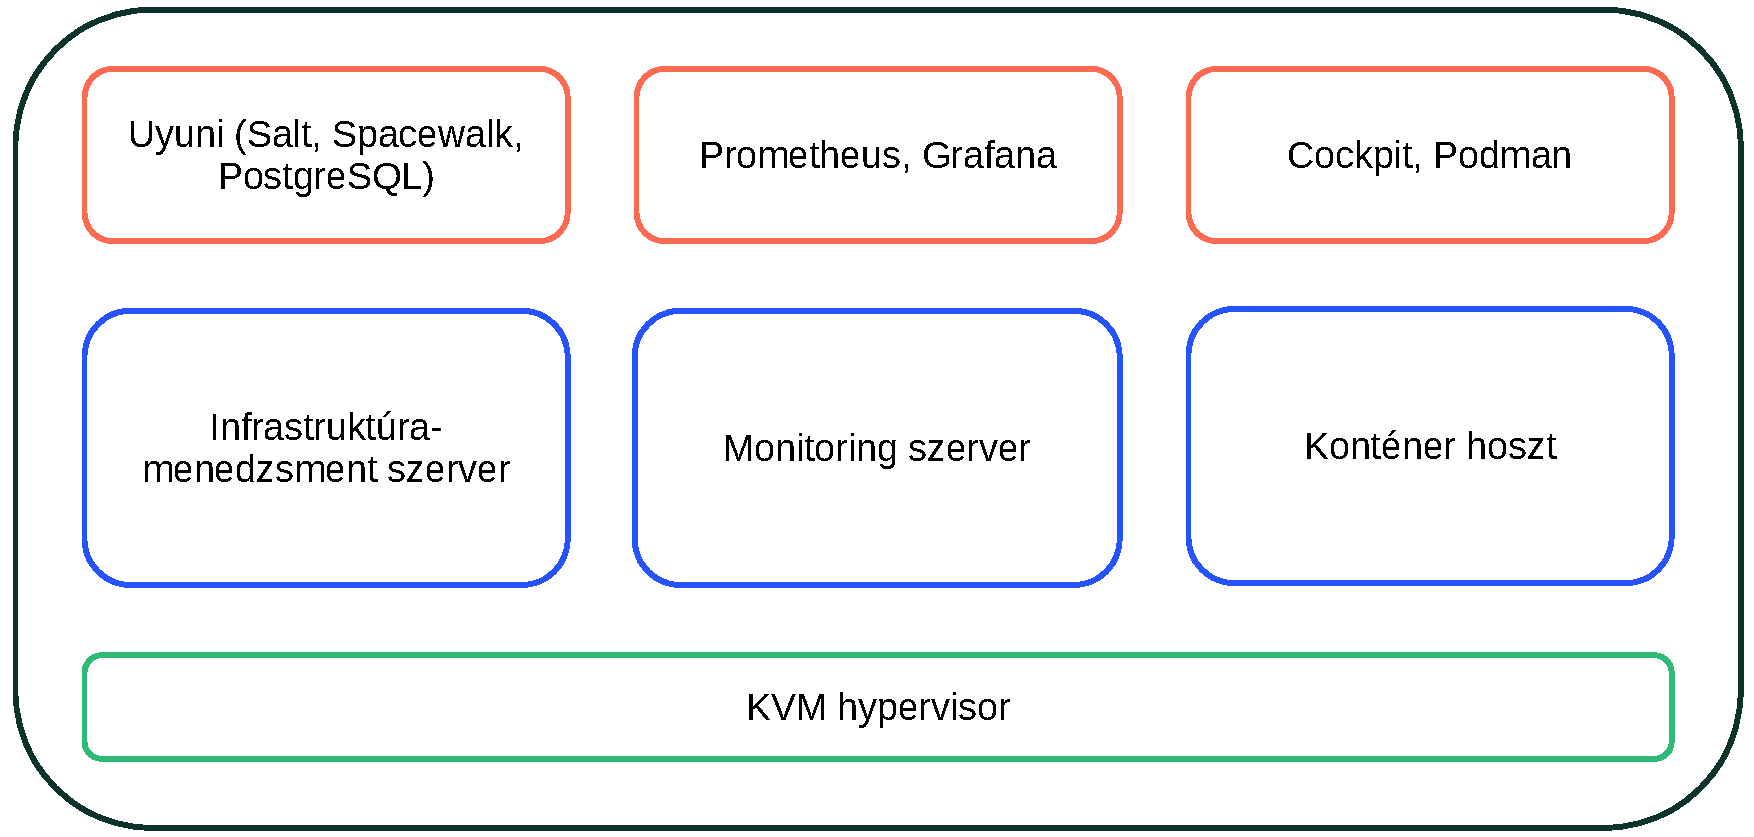
\includegraphics[width=15cm]{figures/architektura.pdf}
	\caption{A tesztkörnyezet tervezett felépítése.}
	\label{fig:test-env-arch}
\end{figure}

\section{Fizikai gép ismertetése}
Ahogy arról \aref{sect:servers} alfejezetben már írtam, a szervergépek több lényeges tulajdonságukban is eltérnek a személyi számítógépektől. A virtualizáció szempontjából legfontosabb ilyen különbségek a processzormagok száma és a memória mennyisége. A tesztkörnyezetet szerettem volna egy ilyen gépen megvalósítani, hogy az ténylegesen a lehető legközelebb állhasson egy valós felhasználási környezethez. Bár a lehetőségeim korlátozottak voltak, sikerült beüzemelnem egy régi, Sun Fire X4450 típusú szervergépet. Ez négy fizikai \acrshort{cpu}-val rendelkezik, mind a négy processzor 6-6 magot tartalmaz, így összesen 24~maggal gazdálkodhattam. Emellett a gép 64~GB memóriával van felszerelve, és egy 1~TB-os \acrshort{ssd}-meghajtó található benne. Ezek mellett a korábban említett hardveres redundancia is megjelenik a gépben: két tápegysége és négy hálózati csatlakozója van, továbbá távolimenedzsment-porttal is rendelkezik, mely lehetővé teszi a szerver távolról történő ki- és bekapcsolását, illetve a rendszernaplók böngészését.

\begin{figure}[!ht]
	\centering
	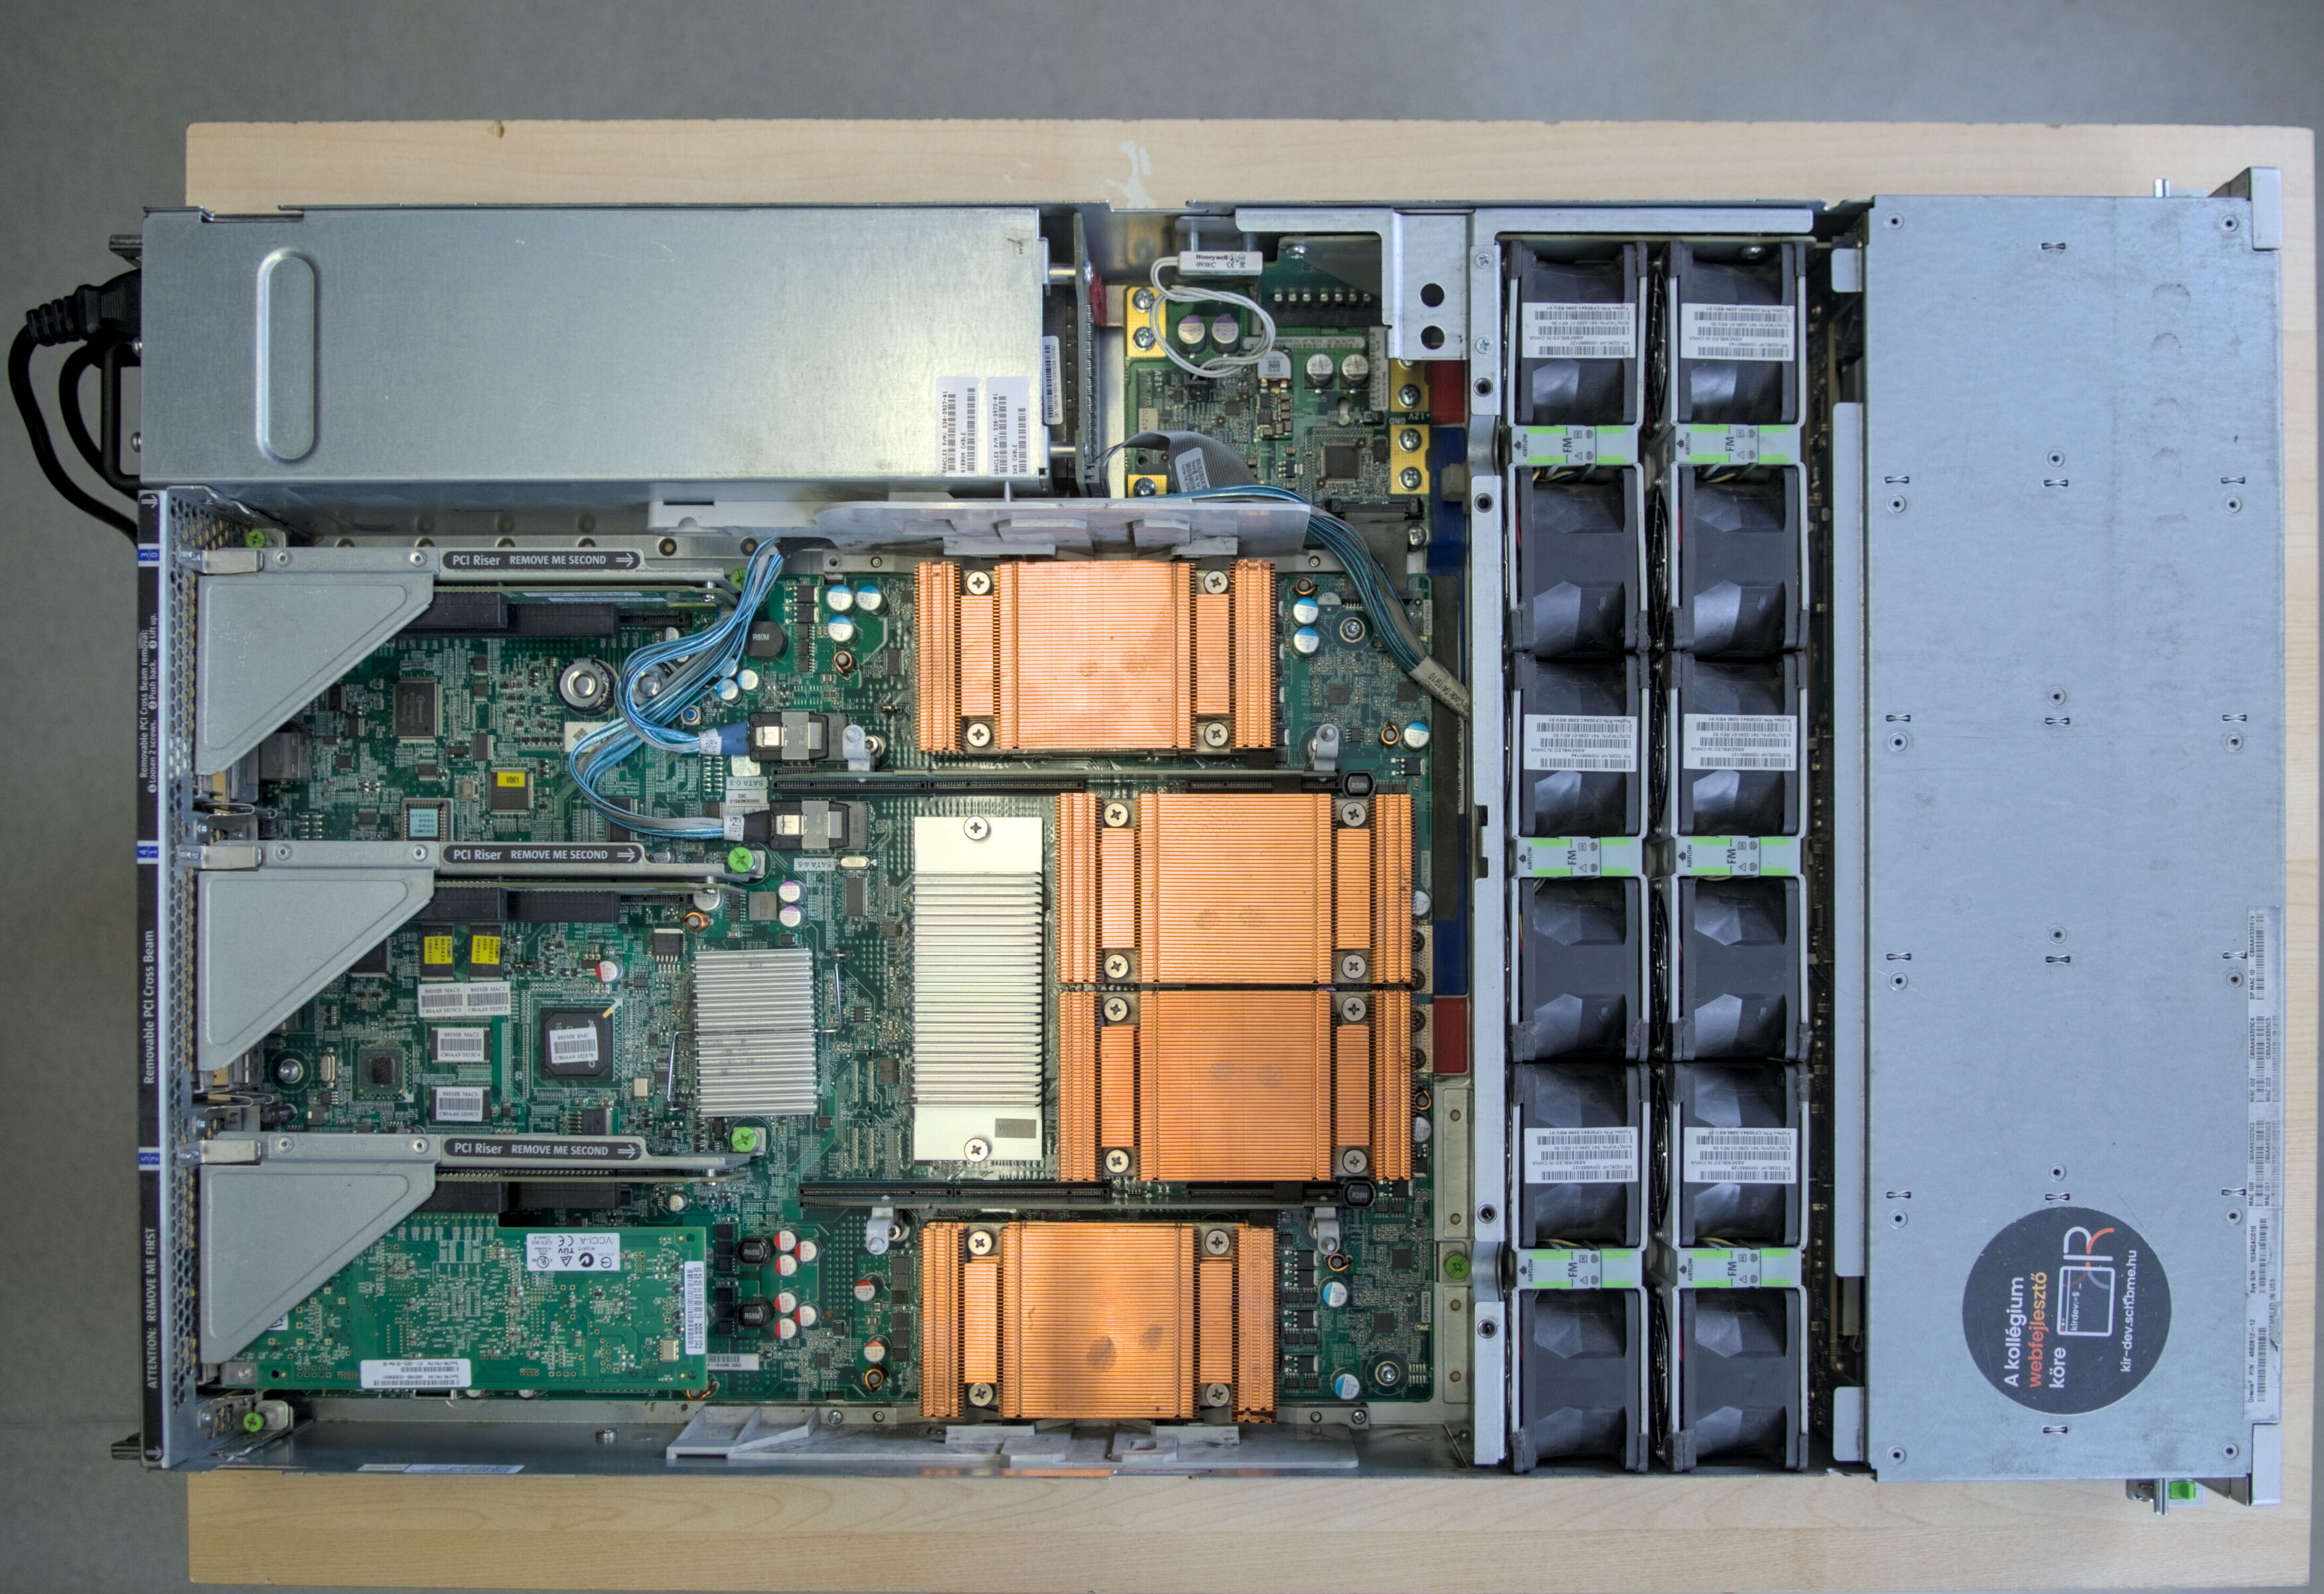
\includegraphics[width=15cm]{figures/szerver.jpg}
	\caption{A tesztkörnyezetben használt fizikai gép. A fotón megfigyelhető a moduláris felépítés, a memóriatálcát eltávolítva pedig a négy különálló \acrshort{cpu} is láthatóvá válik.}
	\label{fig:server}
\end{figure}

\section{Operációs rendszer}
Értekezésemben nagy szerepe lesz a választott operációs rendszereknek, hiszen ezek fognak a virtualizációs rendszer alapjául szolgálni, valamint képesnek kell lennünk a gépek távoli menedzsmentjére is, így mindenképpen olyan megoldásra van szükség, amely jól támogatott a választott infrastruktúramenedzsment-eszköz által. Fontos szempont volt továbbá, hogy a tesztkörnyezet a lehetőségekhez mérten jól képviselje a nagyvállalati környezetben használatos rendszereket, így sok olyan OS-verzió kikerült a lehetőségek közül, amelyek ugyan népszerűek például asztali megoldásként, de egyes nagyvállalati szoftverek (legyen az adatbázismotor, vagy bizonyos eszközvezérlők, driverek) hivatalosan nem támogatottak rajtuk. Emiatt az operációs rendszerek kiválasztása során körültekintően jártam el, több Linux-disztribúció is szóba került, az ezekről született konklúziót itt foglalom össze néhány mondatban.

\subsection{OS-kiválasztás folyamata}
Ahogy \aref{sect:os}. alfejezetben is kitértem rá, a nagyvállalatok elsősorban a Red Hat és a SUSE Linux-disztribúciók közül választanak, hiszen ezeknek a velük együtt járó támogatás és a szoftvercsomagok széleskörű támogatottsága miatt kényelmesebb és hatékonyabb az üzemeltetésük, valamint biztonsági szempontból is kedvezőbbek (például gyorsabban kapnak meg bizonyos frissítéseket, patcheket). Szintén jobban támogatottak ezeken a rendszereken a különböző felhasználásspecifikus modulok, például \acrfull{ha}, live patching (támogatás pl. kritikus kernel biztonsági javítások telepítése a számítógép újraindítása nélkül) és real time computing (valós idejű, nagy időbeli pontosságot igénylő alkalmazások futtatására alkalmas környezet).

A fent ismertetett szélesebb körű támogatottság miatt a tesztkörnyezethez használni kívánt operációs rendszerek köre a Red Hat-re és a SUSE Linuxra korlátozódott. A végső döntésben végül az alábbi szempontok segítettek:
\begin{itemize}
	\item a tesztkörnyezetet szerettem volna egy ökoszisztémán belül tudni mind a virtuális gépeket futtató, mind pedig az azokon futó \acrshort{os}-ek esetében,
	\item könnyebb konfigurálhatóság: mivel több gépet kellett telepíteni, így fontos szerepe volt annak, hogy egy-egy operációs rendszer telepítése milyen bonyolultságú,
	\item a környezetet a költségek minimalizálása mellett szerettem volna létrehozni, így lényeges szempont volt, hogy az adott rendszerhez ne kelljen előfizetést vásárolni, mégis a lehető legközelebb álljon a kereskedelmi forgalomban kapható termékekhez.
\end{itemize}

Mindezek figyelembevételével és korábbi tapasztalataim alapján a SUSE termékcsaládja mellett döntöttem. A támogatással rendelkező, előfizetéses modellt használó nagyvállalati változat mellett szabadon beszerezhető openSUSE operációsrendszer-család megfelelt a tesztkörnyezettel szemben támasztott elvárásaimnak. A rendszer telepítését és a későbbi konfigurációt a YaST keretrendszer segíti, mely számos moduljával (pl. particionálás, hálózati és tűzfalbeállítások) nagyban hozzájárul a gépek könnyebb beállításához, kezeléséhez. A YaST -- mivel szervereken való használatra tervezték, melyek gyakran nem rendelkeznek grafikus felülettel -- \aref{fig:yast-partitioner} ábrán látható megjelenés mellet egy konzolos, GUI-szerű (GUI-like) felülettel is rendelkezik, így a konfiguráció kényelmesen elvégezhető konzolos hozzáférés, például \acrshort{ssh} használata esetén is.

% TODO: yast kép olvashatóság ellenőrzése
\begin{figure}[!ht]
	\centering
	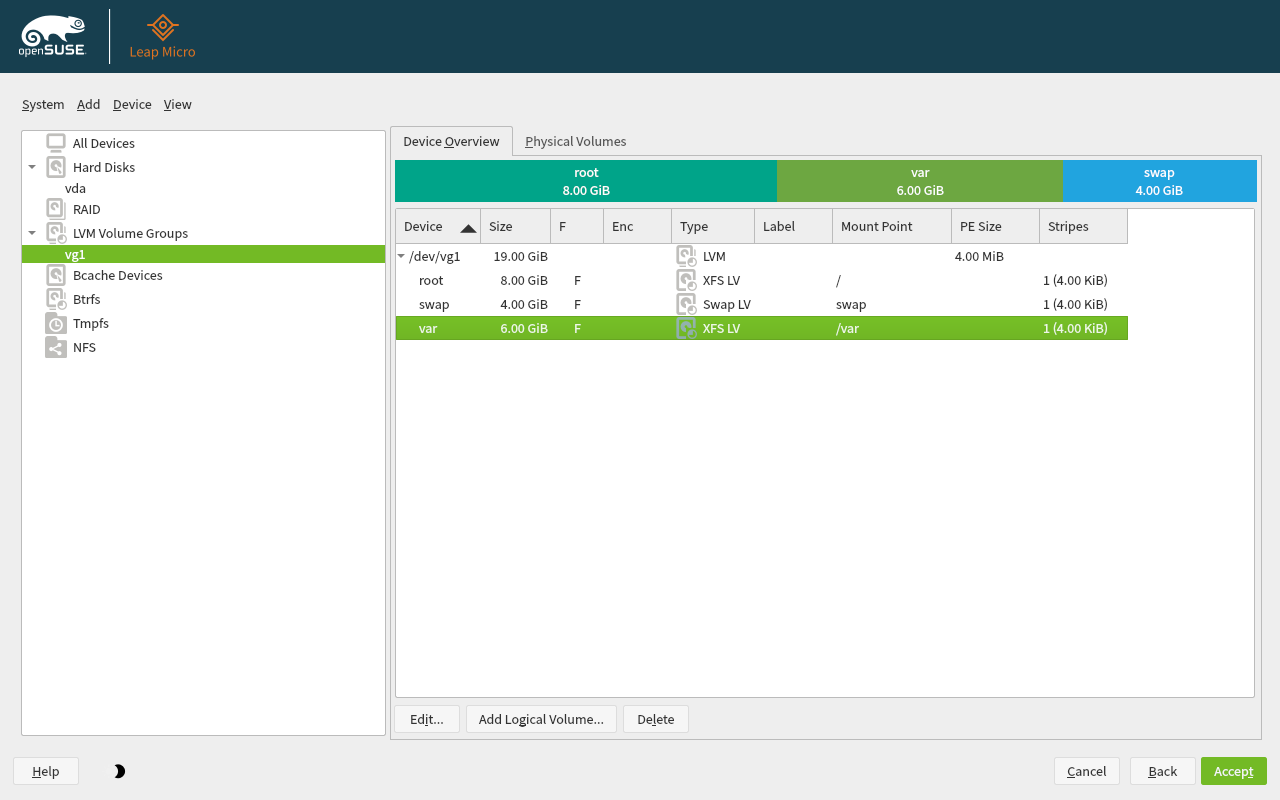
\includegraphics[width=15cm]{figures/yast-partitioner.png}
	\caption{\acrshort{lvm}-kötetek létrehozása openSUSE Leap Micro telepítése során grafikus YaST telepítő segítségével.}
	\label{fig:yast-partitioner}
\end{figure}

Az openSUSE-projekt több operációs rendszert is fejleszt\footnote{\url{https://get.opensuse.org/}}, ezek közül én a tesztkörnyezetben kettőt használtam, melyeket a következő alfejezetekben ismertetek.

\subsubsection{openSUSE Leap}
A Leap egy hagyományos értelemben vett szerver operációs rendszer. Gyakran kap biztonsági frissítéseket, új verziói pedig körülbelül évente jelennek meg. Alapjául a \acrfull{sle} szolgál, melynek előnye, hogy a két rendszer csomagjai binárisan kompatibilisek egymással, azaz egy \acrshort{sle}-rendszerre készített csomag garantáltan használható openSUSE Leap-en is, és fordítva~\cite{openSUSELeap15SP3intro}~\cite{SLE15SP3intro}. Utóbbi előnye, hogy így számos, a közösség (akár a hivatalos openSUSE projekt, akár a felhasználók) által készített csomagot használhatunk a \acrshort{sle}-alapú rendszerünkön is, bár ehhez nem kapunk hivatalos támogatást.

A nagyvállalati rendszerből való leszármazás másik nagy előnye, ami fontos volt számomra a kiválasztási folyamat során, hogy így gyakorlatilag a \acrlong{sle} egy ingyenes verzióját használhatom, mely lényegében teljesen megegyezik a vállalati környezetben használt megoldással, és előfizetés nélkül is kap frissítéseket, így folyamatosan naprakészen tartható. A biztonsági javításokat illetően fontos megjegyezni, hogy a Leap rendelkezik egy olyan csomagforrással (repository) is, mely a \acrlong{sle}-ban is elérhető frissítéseket tartalmazza, így az ott hozzáférhető fontos javításokat is telepíthetjük a Leap-et futtató rendszereinkre~\cite{openSUSELeapSLERepo}.

\subsubsection{openSUSE MicroOS}
A MicroOS egy újfajta megközelítést használó, modern operációs rendszer, mely elsősorban konténerizált alkalmazások futtatásához készült. \Az{\acrshort{os}} előnye, hogy az alap telepítés csak egy minimális szoftvercsomagot tartalmaz, így az erőforrásigénye elenyésző. A MicroOS egy írásvédett (read-only) BTRFS fájlrendszerű gyökérkönyvtárral rendelkezik, melynek előnye, hogy magas szintű támogatást nyújt fájlrendszer-pillanatképek (filesystem snapshots) kezelésére.
Erre a technológiára épít a MicroOS filozófiája: atomi frissítéseket támogat, ami azt jelenti, hogy egy csomag vagy frissítés telepítése során nem az éppen használatban lévő partíció változik, hanem egy új snapshotba kerülnek a módosítások, mely -- amennyiben a módosítás sikeresen lezajlott -- a következő bootolási folyamat során aktívvá válik, és \az{\acrshort{os}} erről kerül betöltésre, így ekkor már használhatjuk a telepített csomagokat. Az atomi frissítések lényege, hogy a módosítások csak akkor lépjenek életbe, ha a teljes folyamat hiba nélkül futott le, azaz például ha egy művelet során a módosítandó 100 csomagból akár csak egy nem tud települni valamilyen hibából eredendően, akkor a teljes telepítés meghiúsul, ezzel elkerülve azt, hogy a rendszer inkonzisztens állapotba kerüljön. A MicroOS ezáltal képes biztosítani azt, hogy a rendszerünk mindig használható állapotban legyen.

A snapshotok fontos tulajdonsága, hogy mindaddig, amíg nem kerülnek törlésre, használatukkal a rendszer bitről bitre visszaállítható abba az állapotba, amiben a pillanatkép készítésekor volt. Ennek nagy jelentősége lehet egy félresikerült rendszerfrissítést követően, hiszen a korábbi állapotra visszaállva a rendszer zavartalanul folytathatja a működést a hiba elhárításáig.
A probléma okának felderítését segíti a snapshotok felcsatolásának lehetősége: ez azt jelenti, hogy a BTRFS fájlrendszer képes arra, hogy a éppen használt partíció mellett az ahhoz tartozó pillanatképeket is felcsatoljuk, sőt, a két állapotot össze is vethetjük a verziókezelő rendszerekben megszokott módon (erre például a YaST beépített támogatással rendelkezik), mely tovább könnyítheti a hiba forrásának felderítését.
% TODO: btrfs diff ábra

A MicroOS különlegességei közé tartozik még, hogy a szerver operációs rendszereknél megszokott konzolos és távoli asztalos elérés mellett egy webes felületet is biztosít a rendszer kezelésére. Ehhez a Cockpit adminisztrációs rendszert használja, mely az utóbbi években egyre nagyobb népszerűségnek örvendő megoldás. A Red Hat disztribúciói például már ezt a rendszert ajánlják a virtualizáció kezelésére a korábban megszokott virt-manager helyett~\cite{RHELDeprecated}.

A Cockpit felülete gyors áttekintést nyújt a rendszer állapotáról, továbbá könnyíti a konténerek létrehozását (\ref{fig:cockpit-container}.~ábra) és kezelését. A fontosabb metrikák (processzor-, memória-, háttértár és hálózathasználat) megtekintése mellett szükség esetén közvetlenül is be tudunk avatkozni a rendszer működésébe, ugyanis a felület egy terminállal is rendelkezik. Továbbá a futó szolgáltatások állapotát is figyelemmel kísérhetjük, valamint a felhasználói fiókokat is kezelhetjük a Cockpit segítségével.

\begin{figure}[ht]
	\centering
	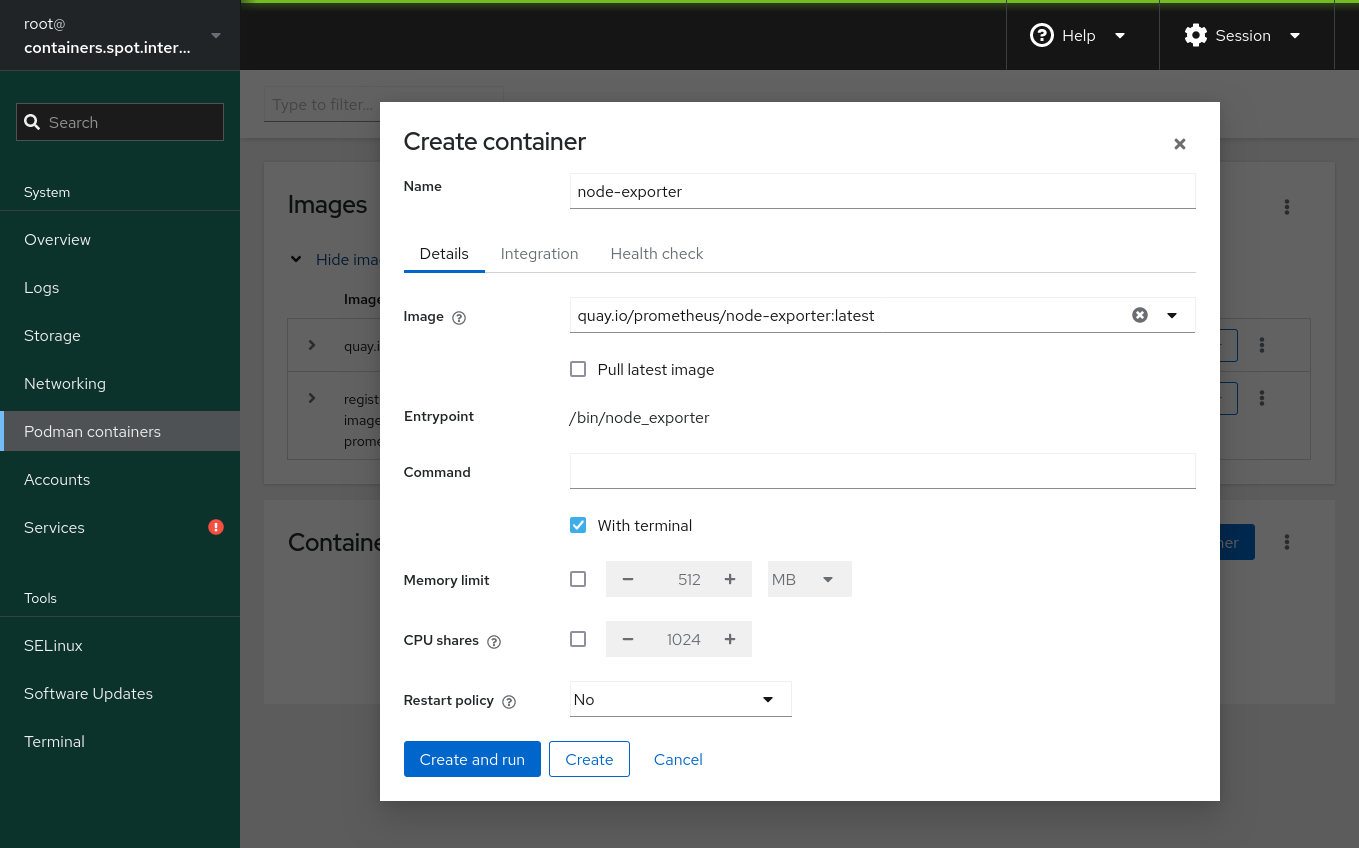
\includegraphics[width=15cm]{figures/cockpit.png}
	\caption{Konténer létrehozása openSUSE Leap Micro-n, a Cockpit webes felületén keresztül.}
	\label{fig:cockpit-container}
\end{figure}

Az openSUSE-projekt kétféle MicroOS-verziót tart karban: a MicroOS-t, mely egy rolling release modellt követ, azaz a rendszer folyamatosan (akár napi szinten) kapja meg a frissítéseket, így több, kisebb verzióugrással tartható karban, míg az openSUSE Leap Micro a \acrlong{sle} Micro kiadási modelljét követi, és a Leap-hez hasonlóan bináris kompatibilitást garantál a két verzió között. A tesztkörnyezethez a stabilitás és kompatibilitás miatt a Leap Micro változatot választottam.

\section{Hálózati topológia}
Az infrastruktúra működésében fontos szerepe van a hálózatnak: a távoli elérésen túl biztosítani kell a szoftvercsomagok elérhetőségét is, valamint a későbbiekben látni fogjuk, hogy a monitoring rendszer is hálózaton keresztül gyűjti az adatokat. Ezek miatt lényeges volt, hogy a gépek tudjanak kommunikálni egymással és a külvilággal. A tesztkörnyezet hálózati felépítését \aref{fig:test-env-network}.~ábra szemlélteti.

\begin{figure}[ht]
	\centering
	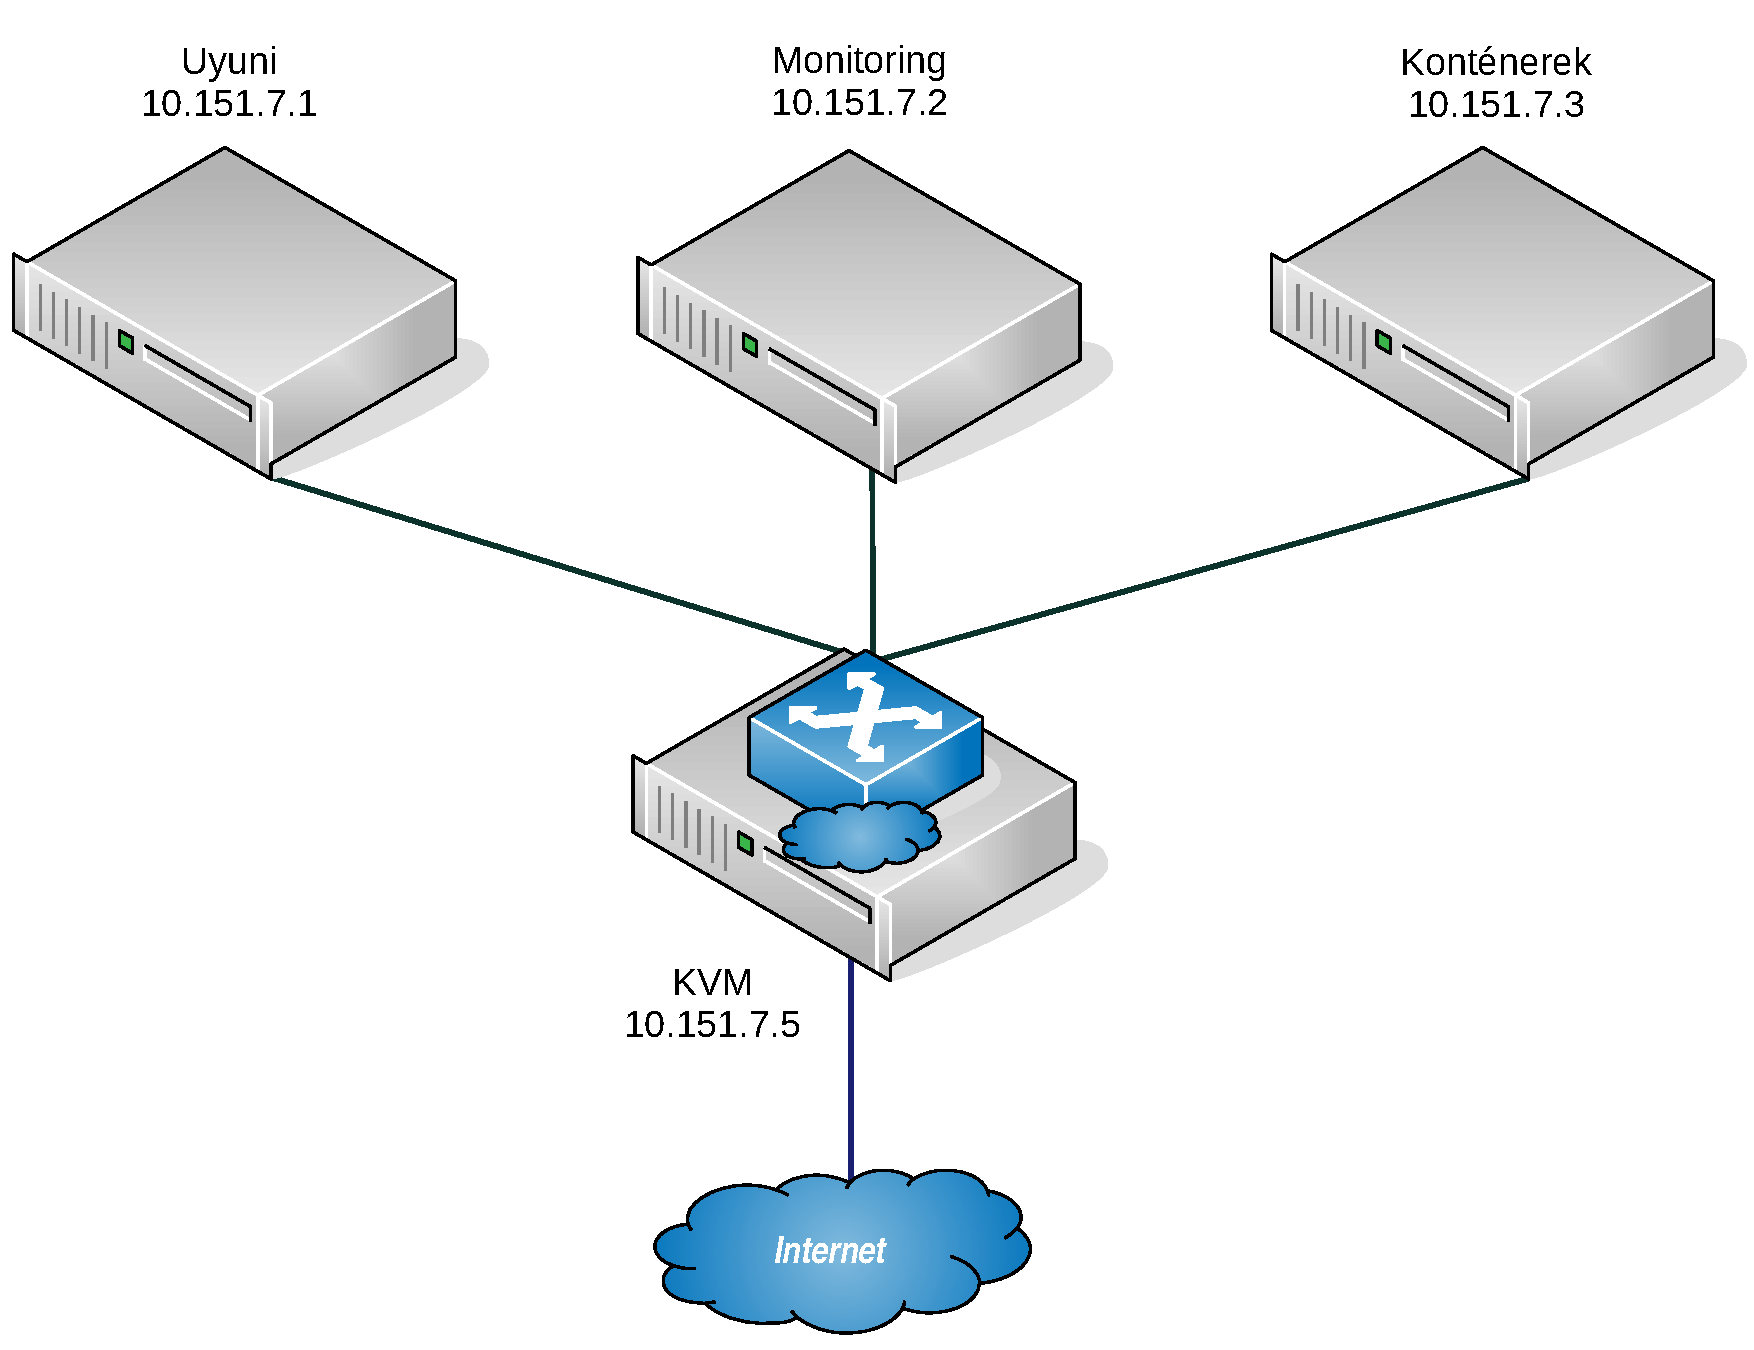
\includegraphics[width=15cm]{figures/halozat.pdf}
	\caption{A tesztkörnyezet hálózati felépítése. Az ábrán nem szerepel a szervergép \texttt{10.151.7.4}-es IP-című menedzsment portja.}
	\label{fig:test-env-network}
\end{figure}

\subsection{Bridge-dzselt hálózati interfész}
\label{sect:net-bridge}
A virtualizált környezetek sajátossága, hogy a virtuális gépek alapesetben egy -- a virtualizációt biztosító szoftver által kezelt -- hálózatra tudnak csatlakozni, a fizikai gép hálózatán nincs lehetőségük kommunikálni. Ez a megoldás általában külön konfiguráció nélkül elérhető, viszont hátránya, hogy a külvilág felé gyakorlatilag láthatatlanná válik a virtuális gép. Bár ez porttovábbítással és a tűzfalbeállítások, valamint az érintett szolgáltatások módosításával orvosolható, a hálózati interfészek bridge-dzselése egy szélesebb körben használható megoldást nyújt.

Egy bridge-dzselt interfész lehetővé teszi a virtuális gépek számára, hogy a gazdagéppel azonos hálózaton kommunikáljanak, azaz ugyanúgy működjenek, mintha minden virtuális gép virtualizált hálózati interfészéhez tartozna egy dedikált hálózati csatlakozó a fizikai gépen, mely egyazon hálózathoz csatlakozik. Ehhez a gazdagép hálózati beállításaiban létre kell hozni egy hálózati híd eszközt, és a használni kívánt interfészt be kell állítani bridge masterként.
Ezeket a beállításokat egyszerűen elvégezhetjük parancssori felületen, illetve a YaST segítségével is (\ref{fig:yast-net-bridge}.~ábra). Az így létrejött virtuális eszköz az OSI-modell szerinti második szinten, az adatkapcsolati rétegben működik a hardveres switch-ekhez hasonlóan~\cite{SUSENetBridge}.

\begin{figure}[ht]
	\centering
	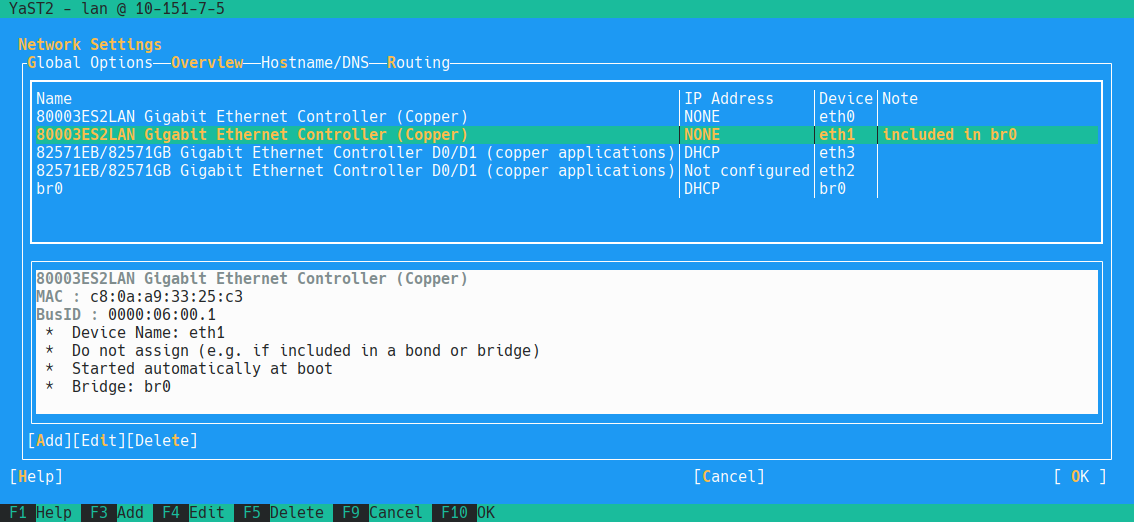
\includegraphics[width=15cm]{figures/yast-br0.png}
	\caption{A tesztkörnyezethez beállított hálózati bridge alapjául szolgáló eth1 fizikai~interfész beállításainak részletei a YaST konfigurációs program parancssori változatában. Látható, hogy az eth1~interfész a br0~bridge eszközhöz van társítva, és előbbihez emiatt nincs hozzárendelve IP-cím.}
	\label{fig:yast-net-bridge}
\end{figure}

\section{Virtualizációs komponensek telepítése}
A tesztkörnyezet szoftveres alapját a virtualizációs megoldások adják. Ebben az alfejezetben ismertetem a fizikai gép előkészítését és a virtuális gépek telepítésének folyamatát, valamint az ezekhez kapcsolódó beállítási lépéseket, kitérve például a particionálás folyamatára és a virtuális gépek terminálos elérésére.

\subsection{Hosztgép konfigurálása}
A virtualizációs környezetet futtató számítógépre az openSUSE Leap 15.5-ös verzióját telepítettem, mely a tesztkörnyezet kialakításakor a disztribúció legfrissebb stabil elérhető változata. A telepítés során a gép szerepének (system role) a szerver opciót választottam. Ez a felhasználási céloknak teljesen megfelelt, hiszen ez a megoldás is egy jól felszerelt operációs rendszert telepít, csak asztali környezet nélkül. Mivel a szervert elsősorban konzolos felületen, \acrshort{ssh}-n keresztül szerettem volna használni, ezért ez nem jelentett gondot. Sőt, a tesztkörnyezet szempontjából előnnyel is járt: a rendszerre nem volt szükséges az asztali környezet működéséhez elengedhetetlen csomagok telepítése, ami nem csak a tárhellyel való takarékoskodásban segített, de a későbbiekben is könnyítette a karbantartási folyamatokat, mert kevesebb csomagot kellett frissíteni és így az esetleges támadási felület (sérülékenységek száma) is kisebb volt. Lényeges azonban megjegyezni, hogy az X11 könyvtár a szerver csomag részeként is telepítésre került, így adott volt a lehetőség X~forwarding\footnote{Távoli szerveren futtatott, grafikus felülettel rendelkező alkalmazások ablakának a kliensgép képernyőjén való megjelenítését lehetővé tevő technológia.} használatára.

A hálózatkezeléshez -- a virtuális gépek hálózati elérését lehetővé teendő -- \aref{sect:net-bridge}.~alfejezetben bemutatott bridge-dzselt hálózati interfészt állítottam be. Ehhez az alapértelmezett beállításokhoz képest annyit kellett módosítani, hogy a bridge-dzselt eszköz a fizikai interfészen keresztül kommunikáljon, illetve hogy a virtualizációs hosztnak kiosztott \texttt{10.151.7.5}-ös IP-címet ne az \texttt{eth1} fizikai interfész kapja meg, hanem az újonnan létrehozott \texttt{br0} eszköz. Ezt követően a számítógép a korábban megszokott módon tudott a hálózaton kommunikálni, viszont lehetővé vált, hogy a virtuális gépek is hozzáférjenek a fizikai gép hálózatához a bridge eszközön keresztül.

A hálózaton kívül a másik lényeges tervezői döntés a logikai kötetek (\acrshort{lvm}) alkalmazása volt. Ez a gyakorlatban azt jelentette, hogy a boot partíció kivételével minden egyéb kötetet \acrshort{lvm}-kötetként hoztam létre. Ennek legfőbb előnye számomra a kötetek méretének rugalmas kezelése volt, melyről \aref{sect:lvm}. alfejezetben írtam bővebben. Emellett lehetőséget biztosít pillanatképek készítésére is, melyek készítése például \acrshort{os}-frissítések előtt lehet releváns, és nagyban megkönnyíti rendszer korábbi állapotának helyreállítást, ha valami hiba jelentkezik a folyamat során. A kötetkiosztás úgy történt, hogy minden virtuális gép kapott egy külön \acrshort{lvm}-kötetet, amit egy egyedülálló tárolóeszközként érzékelt, és ezt használhatta az adatok tárolására, akár további particionálás mellett is.

A kezdetleges konfigurációt követően telepítettem a \acrshort{kvm} \gls{hypervisor}t és a virtuális gépek kezeléséhez szükséges csomagokat. Ehhez openSUSE-disztribúciókon külön ún.~pattern áll a rendelkezésünkre. Ez azt jelenti, hogy nem kell megadnunk minden telepítendő csomagot, hanem elég a \texttt{kvm\_server} és a \texttt{kvm\_tools} pattern-ök telepítése, és ezek automatikusan telepítésre jelölik a teljes értékű \acrshort{kvm}-szerverhez szükséges csomagokat, emellett néhány hasznos segédprogramot (pl. virt-manager, virsh) is magukkal hoznak. Ezen csomagok telepítését követően minden előfeltétel adottá vált a virtuális gépek telepítéséhez.


\subsection{Virtuális gépek telepítése}
\acrshort{vm}-ek telepítéséhez elsősorban a \texttt{virt-install} parancsot használtam. Ez a program lehetővé teszi az összes lényeges paraméter megadását, majd távoliasztal-protokoll használatával (alapértelmezetten \acrshort{spice}, de választhatjuk például a \acrshort{vnc}-t is) megjeleníti a virtuális gép kijelzőjét egy ablakban, melynek segítségével személyre szabhatjuk a telepítést és telepíthetjük az operációs rendszert. A távoli asztalon keresztüli elérés csak a megfelelő környezet, pl. \acrshort{ssh} használata esetén, X~forwardinggal működik. Amennyiben a virt-install nem talál kijelzőt, akkor a telepítés parancssoron keresztül történik. A virt-install sikeres futás esetén egy virtuálisgép-leíró XML-fájlt hoz létre, mely a gép összes paraméterét tárolja~(\ref{lst:virshxml}.~kódrészlet). A későbbiekben a \acrshort{vm} konfigurációjának módosítása esetén ezt a fájlt kell módosítanunk (akár szövegszerkesztővel, akár GUI-n, például virt-manager-rel). A leírófájl a virtuális gép migrációjához is használható.

Azonban még mielőtt a konkrét telepítést elkezdhetnénk, létre kell hoznunk azt a partíciót, melyre a virtuális gép adatai kerülnek. Esetemben ez azt jelentette, hogy az egyes virtuális gépekhez új \acrshort{lvm}-köteteket kellett létrehoznom. Mivel a logikai kötetek számára otthont adó partíciót és a kapcsolódó fizikai kötetet és kötetcsoportot már a hoszt~\acrshort{os} telepítésekor létrehoztam, ezért a~\acrshort{vm}-ek telepítése során elég volt csak egy-egy logikai kötetet~(\acrshort{lv}) létrehoznom, melyhez az \texttt{lvcreate} parancsot használtam~(\ref{lst:lvcreate}~kódrészlet).
Emellett telepítési forrást is meg kellett adni, melyhez én telepítő lemezképeket használtam. Ilyenkor a~\acrshort{vm} telepítésekor fel kell venni egy virtuális CD-meghajtót a géphez, és meg kell adni a telepítési forrás elérési útját.

\begin{lstlisting}[caption=Virtuális gépek logikai kötetének létrehozásához használt parancs.,label=lst:lvcreate]
	lvcreate -L 20G --name kvm-monitoring vg1
\end{lstlisting}

Ezen túl meg kell adni a gép fontosabb paramétereit is (pl. processzorok száma, memória mennyisége), hogy milyen erőforrásokkal szeretnénk telepíteni azt. A tesztkörnyezetben használt gépek telepítése során elsősorban a dokumentációban ismertetett rendszerkövetelményeket vettem figyelembe az erőforrások meghatározásánál, de mivel aránylag sok erőforrás állt rendelkezésemre, így előfordult, hogy a számítási műveletek gyorsítása érdekében a szükségesnél több magot adtam a virtuális gépeknek. Mivel a~\acrshort{vm}-ek konfigurációja szabadon változtatható a későbbiekben is (esetleg a gép újraindítása szükséges az érvényre jutásukhoz), ezért ez nem jelentett problémát a későbbiekben sem. Emellett a~\acrshort{kvm} támogatja a memória és processzor erőforrások \gls{overcommit}-olását is, azaz nem jelent problémát, ha esetleg a fizikai gépen elérhetőnél több \acrshort{cpu}-erőforrást osztottunk ki a virtuális gépek számára, bár ennek használatára a dolgozathoz készített tesztkörnyezetben nem volt szükség~\cite{RedHatKvmOvercommit}.
A tesztkörnyezet egyik virtuális gépének telepítéséhez használt parancsot \aref{lst:virtinstall}.~kódrészlet mutatja be.

\begin{lstlisting}[caption=Virtuális gép telepítése a virt-install segédprogrammal.,label=lst:virtinstall]
	virt-install --name uyuni --memory 32768 --vcpus 12 --cdrom /mnt/openSUSE-Leap-15.5-NET-x86_64-Media.iso --os-variant opensuse15.5 --disk /dev/vg1/kvm-uyuni
\end{lstlisting}

\begin{lstlisting}[caption=Virtuális gép leírófájljának részlete.,label=lst:virshxml]
	<memory unit='KiB'>33554432</memory>
	<currentMemory unit='KiB'>33554432</currentMemory>
	<vcpu placement='static'>12</vcpu>
	<resource>
		<partition>/machine</partition>
	</resource>
	<os>
		<type arch='x86_64' machine='pc-q35-7.1'>hvm</type>
	</os>
	...
	<devices>
		<emulator>/usr/bin/qemu-system-x86_64</emulator>
		<disk type='block' device='disk'>
			<driver name='qemu' type='raw' cache='none' io='native' discard='unmap'/>
			<source dev='/dev/vg1/kvm-uyuni' index='1'/>
			<backingStore/>
			<target dev='vda' bus='virtio'/>
			<boot order='2'/>
			<alias name='virtio-disk0'/>
			<address type='pci' domain='0x0000' bus='0x04' slot='0x00' function='0x0'/>
		</disk>
	...
	</devices>
\end{lstlisting}

A virtuális gép operációs rendszerének telepítése során ki kellett alakítani a kívánt partíciókiosztást, mely a felhasználási körtől függően változott, de alapvetően mindenhol \acrshort{lvm}-alapú kötetkiosztást alkalmaztam. Emellett szükséges volt bizonyos hálózati beállítások (pl.~\acrshort{dns}-szerver címe, gépnév) módosítása is. Ezeken felül és az alapvető adatok~--~mint~például felhasználói fiókok létrehozása, lokalizációs beállítások konfigurálása~--~megadásán túl mást nem volt szükséges átállítani a telepítés során. A sikeres installációt követően foghattam hozzá a virtuális gépeken futó szolgáltatások telepítéséhez, melyeket a következő fejezetekben fogok részletesen ismertetni.
